\documentclass[tikz,border=12pt]{standalone}
% Shared visual language for standalone EMT block diagrams.
\usepackage{amsmath}
\usetikzlibrary{arrows.meta,backgrounds,calc,fit,positioning}

\tikzset{
    emt diagram/.style = {>={Stealth[length=2.4mm]}},
    line/.style        = {semithick, rounded corners=6pt},
    block/.style       = {draw, semithick, fill=white,
                          minimum height=1cm, minimum width=2.3cm},
    hblock/.style      = {block, minimum width=2.24cm, minimum height=1.3cm},
    vblock/.style      = {block, minimum width=1.3cm, minimum height=2.24cm},
    sum/.style         = {draw, semithick, fill=white, circle,
                          inner sep=2.6pt},
    signal/.style      = {circle, fill, inner sep=1.4pt,
                          label distance=3pt},
    sig/.style         = {font=\small},
    pm/.style          = {font=\scriptsize},
    wire jump/.style   = {line,
                          preaction={draw=white, line width=3pt,
                                     line cap=round}},
    enclosure/.style   = {draw, dashed, semithick, rounded corners=4pt},
    operator enclosure/.style = {enclosure, inner xsep=7mm, inner ysep=6mm}
}


\begin{document}
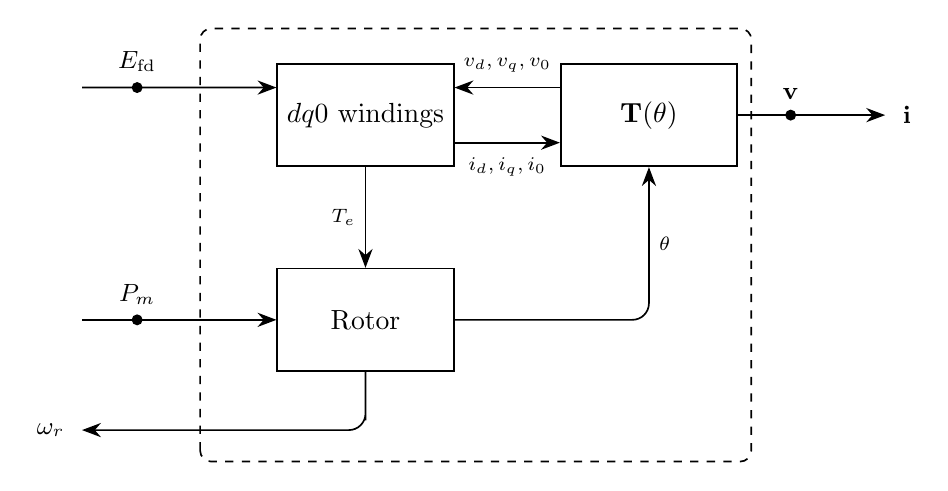
\begin{tikzpicture}[emt diagram]

% ================= Winding, rotor, and Park blocks =================
\node[hblock] (windings) at (0, 1.0) {$dq0$ windings};
\node[hblock] (rotor) at (0, -1.6) {Rotor};
\node[hblock] (park) at (3.6, 1.0) {$\mathbf{T}(\theta)$};

% ================= Terminal voltage and current =================
\node[signal, label={[sig]above:$\mathbf{v}$}] at (5.4, 1.0) {};
\draw[->, line] (park.east) -- (6.6, 1.0);
\node[sig, anchor=west] at (6.7, 1.0) {$\mathbf{i}$};

% ================= Winding to Park coupling =================
\draw[->, line] ([yshift=3.5mm]park.west) -- ([yshift=3.5mm]windings.east);
\node[pm, above] at (1.8, 1.42) {$v_d, v_q, v_0$};
\draw[->, line] ([yshift=-3.5mm]windings.east) -- ([yshift=-3.5mm]park.west);
\node[pm, below] at (1.8, 0.58) {$i_d, i_q, i_0$};

% ================= Rotor coupling =================
\draw[->, line] (windings.south) -- node[pm, left] {$T_e$} (rotor.north);
\draw[->, line] (rotor.east) -| node[pm, right, near end] {$\theta$} (park.south);

% ================= Control inputs and speed output =================
\node[signal, label={[sig]above:$E_\mathrm{fd}$}] (efd) at (-2.9, 1.35) {};
\draw[->, line] (-3.6, 1.35) -- ([yshift=3.5mm]windings.west);
\node[signal, label={[sig]above:$P_m$}] (pm) at (-2.9, -1.6) {};
\draw[->, line] (-3.6, -1.6) -- (rotor.west);
\draw[->, line] (rotor.south) |- (0, -3.0) -- (-3.6, -3.0);
\node[sig, anchor=east] at (-3.7, -3.0) {$\omega_r$};

% ================= Model enclosure =================
\draw[enclosure] (-2.1, -3.4) rectangle (4.9, 2.1);

\end{tikzpicture}
\end{document}
